\documentclass{article}

\usepackage[normalem]{ulem}
\usepackage{fancyhdr}
\usepackage[parfill]{parskip}
\usepackage{tikz}
\usepackage{pgfplots}
\usepackage{multicol}
\usepackage[version=3]{mhchem}
\pagestyle{fancyplain}

\pgfplotsset{compat=1.7}

\title{Atomic structure}
\author{Todd Davies}
\date{\today}

\begin{document}

\rhead{Atomic structure}
\lhead{\today}

\maketitle

\section*{Alpha particle scattering and the nucleus}
\thispagestyle{empty}

Ernest Rutherford was a scientist studying at Cambridge university. He did an
experiment that involved firing $\alpha$ particles at gold foil. He noticed that
most of the particles passed straight through, while very few bounced back or
were deflected. He concluded that most of the atom is empty space, and the
nucleus is very small.

\section*{The simple atomic model}

Rutherfords idea of how the atom was structured was quickly accepted and soon
after, the proton was discovered. However, the proton was too small to account
for all the mass of the atom, which resulted in the discovery of the neutron. It
was easy to work out that the neutrons and protons were situated in the center
of the nucleus and the electrons orbited in a cloud around it.

\section*{Nucleons and electrons}

An atom can be described by the particles that it contains. The basic set of
particles that define atoms are well known, and are as follows:

\begin{center}
 	\renewcommand{\arraystretch}{1.2}
	\begin{tabular}{l|l|l}
		{\bf Particle} & {\bf Relative mass} & {\bf Charge} \\ \hline
		Proton & 1 & +{\it e}\\ \hline
		Neutron & 1 & 0\\ \hline
		Electron & $\frac{1}{1836}$ & -{\it e}
	\end{tabular}

\end{center}

\textit{N.b. Protons and neutrons are often refered to as Nucleons, since they
usually reside in the nucleus of atoms.}

\subsection*{Nuclear notation}

There is a specific notation for writing down what an atom is composed of, it
looks like this:

\[
	\ce{^{\textrm{\it Nucleon number }}_{\textrm{\it Proton number }} X}
\]

\subsection*{Isotopes}

An isotope of an element contains a different number of {\it neutrons} to the
element. This means that it's mass is different and the nucleus of the atom is
potentially unstable. However, it still has the same amount of electrons in it's
outer energy level, so the interactions between it and other atoms are the same.

\section*{Forces in the nucleus}

It is suprising that the nucleus doesn't blow apart, since it is made up of
positive and neutral particles and no negative particles. However, there are
more forces at work inside the nucleus that mean it doesn't just fall apart as
expected.

The force that counteracts the electrostatic forces in the nucleus is called the
{\it strong force}. It only acts over very short distances ($10^{-14}m$) and the
magnitude of the force is related to the seperation between the nucleons.

This graph shows how the strong force changes with distance:

\begin{center}
	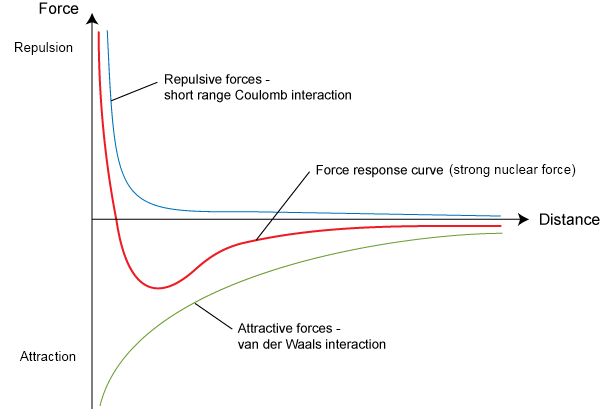
\includegraphics[scale=0.5]{force_graph}
\end{center}

\subsection*{Padding with neutrons}

The strong force still doesn't explain why neutrons are present in the nucleus.
The strong force should act between the protons to keep them bound together,
yes?

In actual fact, the strong force acts only once between each pair of protons
(since it only acts over a distance equal to the radius of a proton). On the
other hand, electrostatic attraction acts over a large distance, so each proton
doesn't just repel the proton next to it, but also repells all of the protons
that it is near to. The combined electrostatic repulsions are greater than the
strong force.

This explains why neutrons are present in the atom. They increase the distance
between the protons so the electrostatic repulsion between them is reduced, yet
they are also affected by the strong force. This has the effect of balancing the
force in the atom and stableising the nucleus. This is also why isotopes with
the incorrect number of neutrons are usually unstable.

\section*{Families of particles}

There are two classes of sub-atomic particles that we use, leptons and hadrons.

An easy way to remember the families is to remember that the word lepton in
Ancient Greek means {\it light}, while hadron means {\it bulky}.

\subsection*{Leptons}

Particles that are unaffected by the strong force are leptons. There are twelve
leptons altogether, since each of the 'main' three (the electron, the muon and
the tau) has an associated neutrino and they all have antiparticles.

\subsection*{Hadrons}

Particles that are affected by the strong force are hadrons. Hadrons are best described by another class of fundamental particle, quarks, so I'll describe them first.

\subsection*{Quarks}

A quark is a type of funadmental particle, they are strange since they can never
exist in isolation. Quarks always combine to form heavier particles, the
hadrons. There are twelve different types of quark (six quarks and six
antiquarks) as follows:

\begin{center}

	\renewcommand{\arraystretch}{1.2}
	\begin{tabular}{|l|c|c|c|c|}
		\hline
		Quark & Symbol & Charge (in units of $e$) & Baryon number & Strangness \\ 
		\hline

		Up & $u$ & $\frac{2}{3}$ & $\frac{1}{3}$ & 0 \\

		Down & $d$ & $-\frac{1}{3}$ & $\frac{1}{3}$ & 0 \\

		Strange & $s$ & $-\frac{1}{3}$ & $\frac{1}{3}$ & -1 \\

		Charm & $c$ & $\frac{2}{3}$ & $\frac{1}{3}$ & 0 \\

		Top & $t$ & $\frac{2}{3}$ & $\frac{1}{3}$ & 0 \\

		Bottom & $b$ & $-\frac{1}{3}$ & $\frac{1}{3}$ & 0 \\

		\hline

	\end{tabular}

\end{center}

{\it N.b. Antiquarks have a dash above the symbol that represents them (e.g. an
Antiup has the symbol $\bar{u}$), have a charge opposite to the charge of the
normal version of them and have the same mass as their normal version.}

\subsection*{Back to hadrons}
So when quarks combine, they form hadrons. For example:

\begin{itemize}
	
	\item A proton is made of two up quarks and a down quark ($u$ $u$ $d$).

	\item A neutron is made of one up quark and two down quarks ($u$ $d$ $d$).

	\item A pi$^+$ meson is made of an up quark and a down antiquark ($u$
	$\bar{d}$).

	\item A phi meson is made of a strange quark and an antistrange quark ($s$
	$\bar{s}$)

\end{itemize}

The properties of any hadron are the sum of the properties of the quarks from
which it is made. For example, to find the charge of a proton, we add up the
charges of two up quarks and a down quark ($\frac{2}{3}+\frac{2}{3}+-\frac{1}{3}
= 1$).

When hadrons interact, all the values for the quantities of their
component quarks (charge, baryon number, strangeness, charm, bottomness and
topness) are conserved.

\section*{The evidence for quarks}

Isolated quarks have never been detected, however there is evidence for their
existance.

Electron diffraction can be used to study matter on an atomic and sub-atomic
scale. Electrons are accelerated at high velocities and, behaving like waves are
diffracted by the particles in the target. The pattern of these diffracted
electrons is then analysed to determine the size and shape of the particles.

Scientists have used this method to analyse protons, the results of which
suggest that protons have an internal structure, and the particles that make up
the structure have various charges that are fractions of $e$.

%TODO:Questions!
\end{document}